\documentclass[11pt, english, a4paper, twoside]{article}

\usepackage[utf8]{inputenc}
\usepackage[main=english]{babel}
\usepackage{url}
\usepackage[nottoc]{tocbibind}
\usepackage{ifthen}
\usepackage[hidelinks]{hyperref}
\usepackage{graphicx}
\usepackage{listings}
\usepackage{caption}
\usepackage{subcaption}

\graphicspath{ {figures/} }

\usepackage[style=iso-numeric, abbreviate=true]{biblatex}
\usepackage{csquotes}
\addbibresource{bibliography.bib} 

\newcommand{\reporttitle}{Distribution of Components in Event-Driven Sensor Networks} 
\pagestyle{myheadings}
\markboth{\reporttitle}{Software Architecture 2022/23, FIIT STU}

\title{\reporttitle}
\author{Bc. Miroslav Hájek} 
\date{Faculty of Informatics and Information Technologies\\
      Slovak University of Technology in Bratislava\\[6pt]
      December 14, 2022}


\begin{document}

\maketitle

\begin{abstract}
Smart building automation and specifically intelligent illumination with IoT are deemed to be a highly heterogeneous environment. Vendors provide functionality that is expected to be interoperable. Lately, standards and guidelines have been put in place to enable implementation flexibility and at the same time define uniform interfaces among the components. Communication between sensors and actuators is event-based with an emphasis on low latency and robust fault handling therefore physical placement of service is to be thoroughly considered. The distributed architectures in a smart building control: CONDE and SorBet are compared to extract important conceptual design decisions. The demo application in Rust language is developed according to the leading standard for the internet of lights OpenAIS. The challenges in design and development are discussed toward achieving compliance with reference architecture specification. We discover that group membership forming and asynchronous message coordination are the most critical choices to get right when varying deployment strategies in the sensor network.
\end{abstract}

\section{Introduction}
Artificial lighting in large office spaces, administrative, and public buildings is no longer about just wiring lamps to a source of electricity through power switches. Although at first look it may seem that way. Trends in energy efficiency and calls for more personalization of these places required to put complex smart measures in effect to satisfy the requirements of building owners, managers, and its inhabitants which can be contradictory at times,  such as optimal power consumption and user preferences. 

However, the objectives remain to be uniform and bright illumination of rooms, light color matching to outside conditions, and possibly daylight incorporation to overall scenery or even its harvesting. It is also desirable that possibly elaborate control mechanisms are transparent as much as possible.

The report further deals in Section~\ref{lighting-control} with the fundamental components of lighting control through the lens of event messaging. Then, the wider context of cooperation inside building management and automation systems is dissected in Section~\ref{bms}. The significant parts of the reference standard for intelligent luminaries are summarized in Section~\ref{openais}. In Section~\ref{demoapp} the implementation is evaluated of a simulation application for distributed lighting. Finally, Section~\ref{related-work} provides related work and Section~\ref{conclusion} summarizes our efforts and proposes the possible next research steps.

\section{Lighting control in smart buildings}  \label{lighting-control}
The feedback loop of the lighting system (fig.\ref{fig:feedback-control}) integrates within the controller settings for the desired amount of light in the chosen place, the observed situation based on sensory inputs, and general parameters for human interface behavior. The result is simply the intensity of light fixtures subject to illumination distribution algorithms. 

Ultimately, the sensors that have impact on the lighting conditions are push buttons, levers, and presence, color, or illumination sensors. Based on their evaluation by the control unit, actuators are affected, which are mostly dimmable or colorized lights. This process can also take blinds into account with some caution, because they affect the indoor temperature.

\begin{figure}
	\centering
	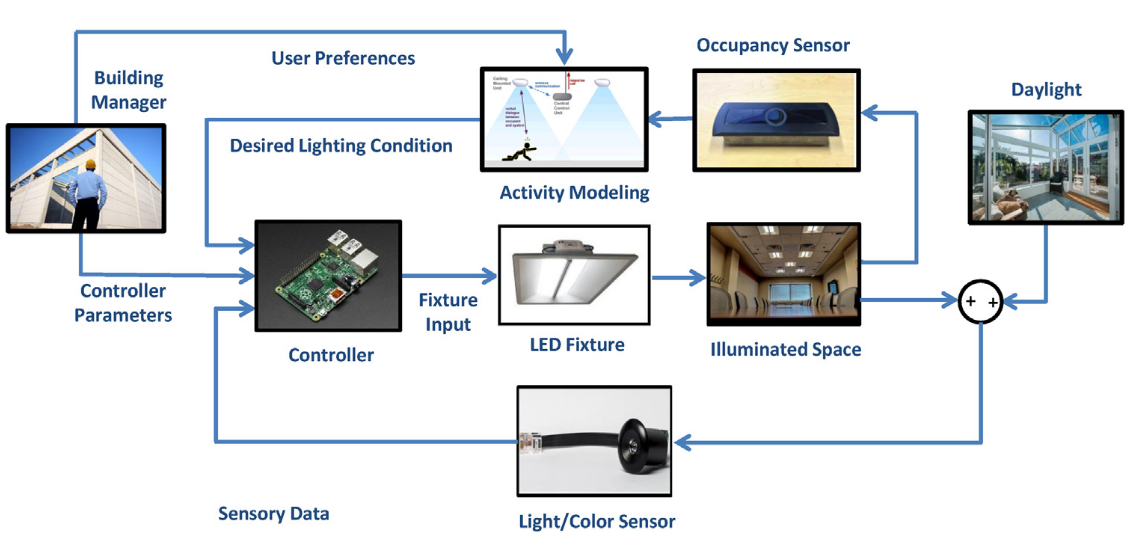
\includegraphics[width=0.8\textwidth]{Feedback-control-loop.png}
	\caption{Elements of lighting control feedback loop \cite{imam_experimental_2016}}
	\label{fig:feedback-control}
\end{figure}
\begin{figure}
         \centering
         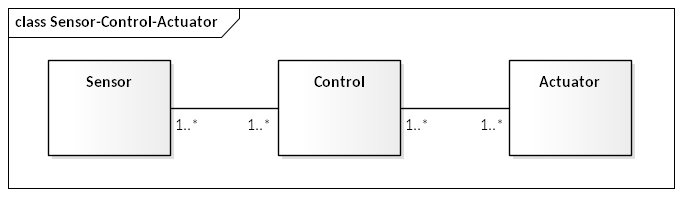
\includegraphics[width=0.8\textwidth]{Sensor-Control-Actuator.png}
         \caption{Sensor-Contol-Actuator model}
         \label{fig:sensor-actuator-model}
\end{figure}

In order to interconnect independent sets of light fixtures in large quantities within the whole building, and maintain resiliency by containing faulty states in relatively isolated logical divisions, simpler bus architectures would not suffice. Lights can be organized as any other common distributed system. The discriminant criterion is the placement of key objects into physical devices. Here, we abide by the typical model consisting of sensors connected to control units that determine actuators' conduct (fig.\ref{fig:sensor-actuator-model}). These three fundamental components can be organized as follows \cite{wen_intelligent_2018}:
\begin{itemize}
	\itemsep0em 
	\item \textbf{Centralized}: Singleton controller exists in the design. All sensors and all light fixtures are dependant on it (fig.\ref{fig:centralized-arch}). Ease of installation and use is counterweighted by the fact that a single point of failure is created for an operation phase.
	\item \textbf{Decentralized}: The polar opposite of centralized apporoach where each light fixture has all components it needs for proper functioning (fig.\ref{fig:decentralized-arch}). Each node is self-reliant but at the cost of high duplication of responsibility. In principal, there is no coordination between any two lights which is a very difficult constraint to apply in practice.
	\item \textbf{Distributed}: It is the compromise between two previous approaches. A disadvantage of decentralized control is solved by introducing some form of local communication between lights (fig.\ref{fig:distributed-arch}). Still, the number of sensors can be further optimized, but then we lose independence for each node and have to think about groups of nodes instead.
\end{itemize}

\begin{figure}
	\centering
     \begin{subfigure}[b]{0.45\textwidth}
         \centering
         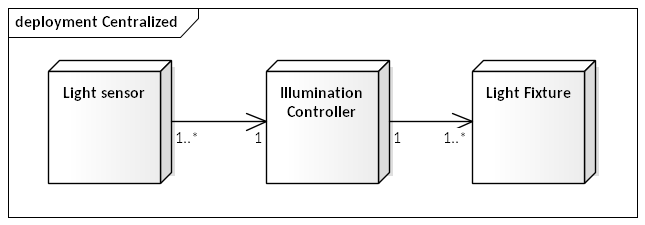
\includegraphics[width=\textwidth]{Centralized-arch.png}
         \caption{Centralized}
         \label{fig:centralized-arch}
     \end{subfigure}
     \hfill
     \begin{subfigure}[b]{0.45\textwidth}
         \centering
         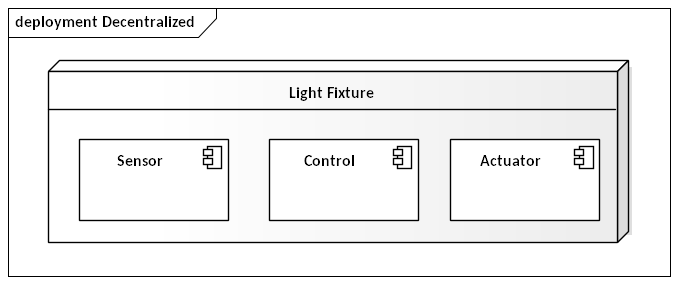
\includegraphics[width=\textwidth]{Decentralized-arch.png}
         \caption{Decentralized}
         \label{fig:decentralized-arch}
     \end{subfigure}
     \hfill
     \begin{subfigure}[b]{0.35\textwidth}
         \centering
         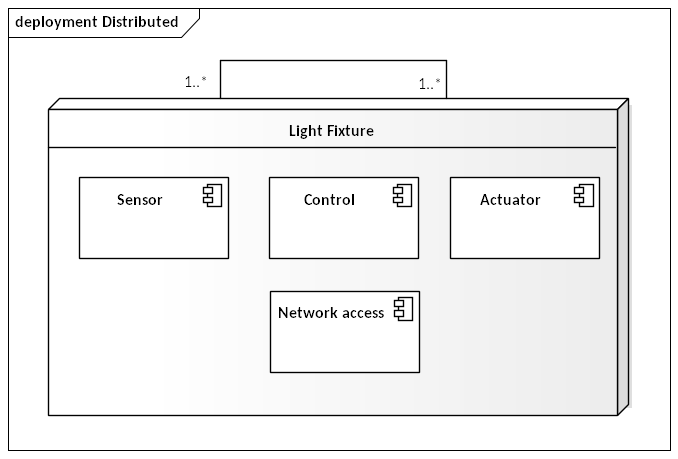
\includegraphics[width=\textwidth]{Distributed-arch.png}
         \caption{Distributed}
         \label{fig:distributed-arch}
     \end{subfigure}
     \caption{Deployment of components from Sensor-Contol-Actuator model}
\end{figure}

No matter the high-level composition of basic structural blocks, the exchange of status and action messages is an important part of wireless sensor-actuator network (WSAN) linking components together. Event-based messaging system is traditionally employed because of on-demand use case for lighting. Activation of communication flow depends on the request given to the publisher causing the emission of a message to the predefined channel towards subscribers (fig.\ref{fig:event-messaging}). 

The details of routing methods can vary based on design decisions. \textbf{Message broker} versus \textbf{message bus} are two considerable options \cite{cristea_distributed_2011}. After the selection of backbone interconnect, the choice of the networking protocol stack is no less important. Mechanisms present in lower layers of the OSI model can be even regarded as a manifestation of either broker or bus. As is the case with IP multicast where network routers can effectively implement event redistribution but they lack buffering capabilities, e.g. holding on to the queue of the latest messages per group. 

\begin{figure}
	\centering
	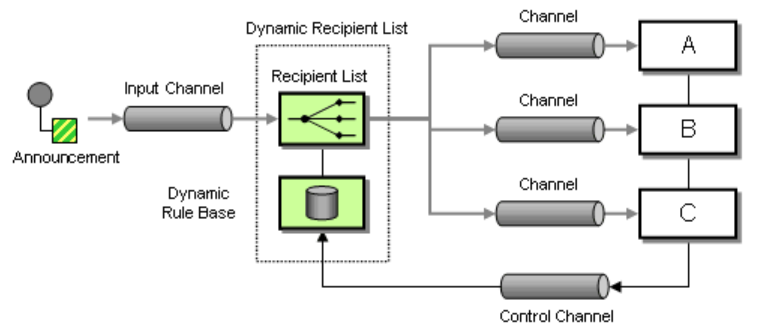
\includegraphics[width=0.7\textwidth]{messaging.png}
	\caption{Messaging \cite{cristea_distributed_2011}}
	\label{fig:event-messaging}
\end{figure}

Another way to look at interactions between components in WSAN is with the use of \textbf{GoF behavioral design patterns}. It is not an exact representation and more of an abstraction, because we do not deal here with objects and classes per se in the sense of an object-oriented paradigm. In this case, \emph{mediator} and \emph{observer} patterns are combined. In event messaging, the role of the mediator is to provide a common element onto which nodes can be attached, previously we referred to this component as broker or bus. At the same time mediator connects components assuming roles of publisher and subscribers, or in the original parlance as subject and observers.

The lighting system can be also understood in terms of \textbf{Event-driven Service Oriented Architecture} (SOA). An event can trigger the invocation of a service or even multiple services. In turn, service execution can produce new events. For example, a person entering the room gets registered by the presence sensor which sends an event to turn on the lights and at the same time notifies the illumination sensor to send its measurement as another event to set adequate light intensity. Another strategy is that lights themselves generate an event to request actual room illumination from the outside. Therefore components mentioned are services because they can execute requested actions and report their status for monitoring purposes. One must be careful about properly chaining command invocations to avoid infinite loops.

\section{Buliding Management Systems IoT architectures} \label{bms}
Modern lighting control usually does not stand on its own, but it is part of a larger building management system (BMS) or building automation system (BAS). The BMS is responsible for sensing the environment inside of the building, on the perimeter, and in the near surroundings whilst integrating various subsystems such as heating, ventilation, entrance access, safety and security appliances, etc. BMS makes decisions on the bases of sensory inputs and acts transparently to the end user.

Many BMS's are integrated into buildings' structural core during the construction phase. Therefore it is usually provided as is with proprietary technology, with small or no regard for scalability or compatibility requirements. Wired communication surpasses in usage wireless transceivers, so new devices depend upon human intervention to configure them. These systems are usually administered and controlled in a centralized manner which we consider mainly disadvantageous for reasons already mentioned.

Next, we compare two BMS architectures found in the literature: CONDE and SorBet. This provides a context where smart lighting fits into the overall building automation and gives us a clearer notion of what to consider alongside subsystem deployment.

\subsection{CONDE Architecture}
A Control and Decision-Making System is a decentralized system for decision and control in smart building applications. Unlike similar solutions, it fully operates among the nodes of WSAN which reduces response time and energy usage compared to centralized architectures \cite{farias_control_2013}. 

\begin{figure}
	\centering
	\begin{subfigure}[b]{0.6\textwidth}
		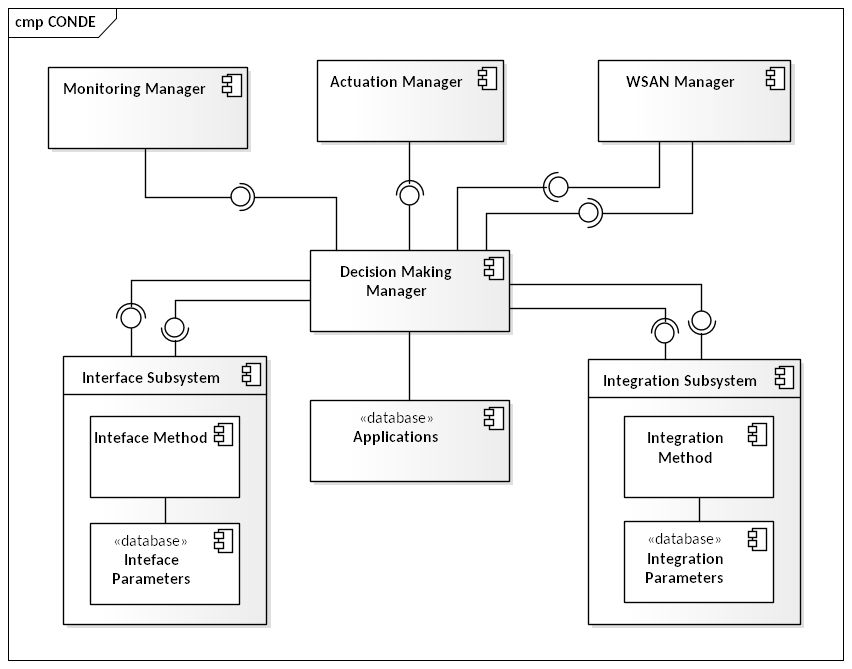
\includegraphics[width=\textwidth]{CONDE.png}
		\caption{Connections between components}
		\label{fig:conde-connections}
	\end{subfigure}
    \hfill
    \begin{subfigure}[b]{0.35\textwidth}
		\centering
		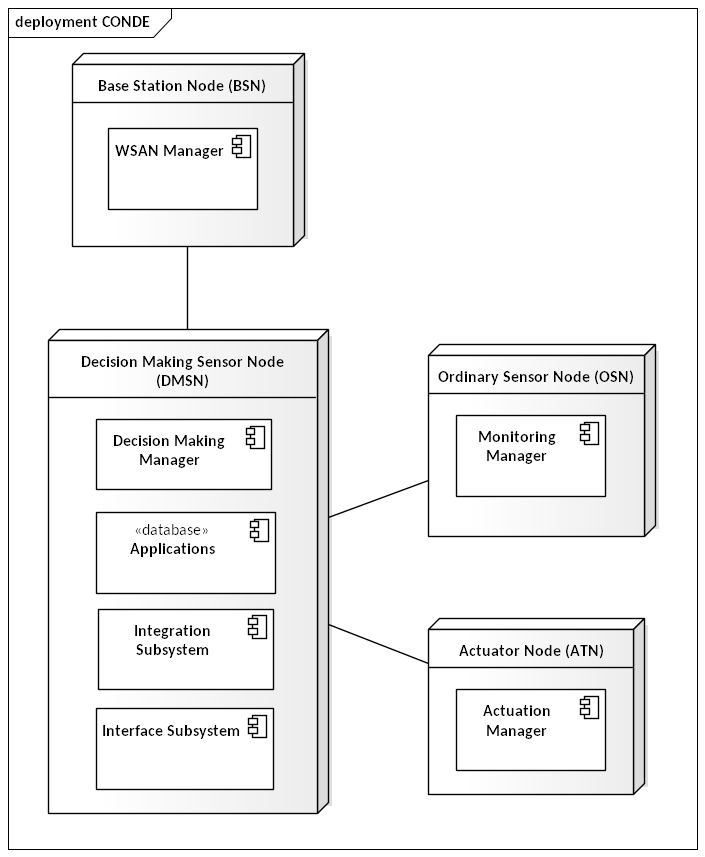
\includegraphics[width=\textwidth]{CONDE-deployment.png}
		\caption{Deployment to WSAN}
		\label{fig:conde-deployment}
	\end{subfigure}
	\caption{System components in CONDE \cite{farias_control_2013}}
	\label{fig:conde}
\end{figure}

We shall notice that fundamental elements of the control feedback loops are present in CONDE too (fig.\ref{fig:conde-connections}). The \emph{Monitoring manager} is responsible for gathering measurements as ordered by the \emph{Decision-making manager} which matches the role of the sensor object. One might recognize the \emph{Actuation manager} as indispensable for performing the solved procedure of steps and identical to the actuator in the basic layout. The two most common event notification scenarios are illustrated in communication diagram (fig.\ref{fig:conde-communication}). 

The rest of the architecture confronts the rules for building equipment behavior with the occurring combinations of situations. These rules are statically predefined in associated databases. Independently for each application, the course of action based on sensor data is dictated by the \emph{Interface subsystem}. However, because of CONDE's purpose in coordinating various aspects of building operations, there might be contradictory decisions from elsewhere. Therefore \emph{Integration subsystem} considers priority and other set factors and determines what should the actuation manager ultimately do \cite{farias_control_2013}. Monitoring and external control should not be neglected so the decision-making manager uses the \emph{WSAN manager} to satisfy those requirements.

In the WSAN not all nodes should be created equal. Naturally, more numerous monitoring and actuator managers are allocated Ordinary Senor Nodes (OSN) and Actuator Node (ATN) respectively (fig. \ref{fig:conde-deployment}). OSNs and ATNs are located close to the devices they act upon. Controller functionality is concentrated inside Decision Making Sensor Node (DMSN). The DMSNs are responsible for logical areas such as floors, halls, or large rooms. In contrast, Base Station Node (BSN) housing the WSAN manager is present in most cases as the only unit in the system, optionally with a fallback.

\begin{figure}
	\centering
	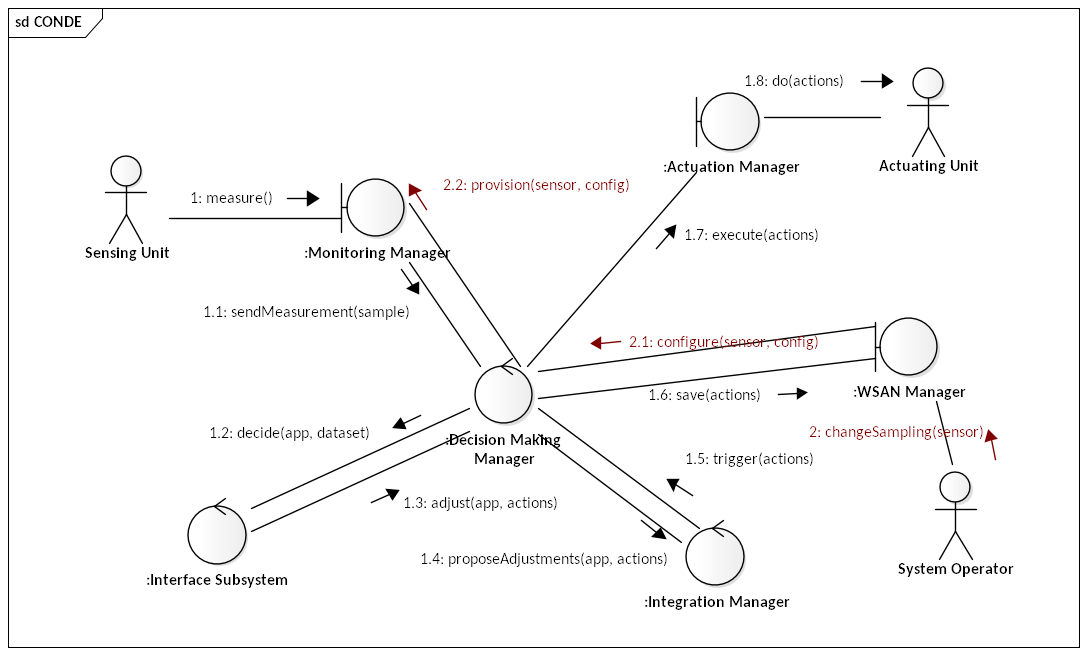
\includegraphics[width=0.9\textwidth]{CONDE-communication.png}
	\caption{Sensor measurement and evaluation}
	\label{fig:conde-communication}
\end{figure}

\subsection{SOrBet Architecture}
SOrBet architecture was created as part of the Marie Curie IAPP project to help the independent living of elderly and disabled people by embedding intelligence in their homes to tail surroundings to their preferences autonomously. Opening windows to freshen the air, turning off unused appliances, and opening doors posing as obstacles are just a few examples of everyday activities these systems handle \cite{tragos_iot_2015}.

The target audience for ambient assisted living (AAL) systems is slightly different from regular BMS, but in terms of heterogenous device infrastructure, timeliness, and data reliability they are not so dissimilar. The functional components are derived from the framework set out by the Architectural Reference Model (ARM) of IoT-A using security and privacy concepts from the RERUM project \cite{rerum}.

The design composition follows a standard IoT pattern to distinguish between the real and virtual world. Hardware device firmware, its configuration, and guarantees of efficient service providing are ensured by the physical layer (fig.\ref{fig:sorbet}). Virtualization deals with making sure there is a uniform interface and other utilities know which services are available. Then the step up is provided by automation layers to enhance the devices with self-learning capabilities which means continuously adapting to observed regularities in routines. The application layer provides means of deploying IoT applications interested in SorBet services at hand. The necessities of all layers are security and configuration.

\begin{figure}
	\centering
	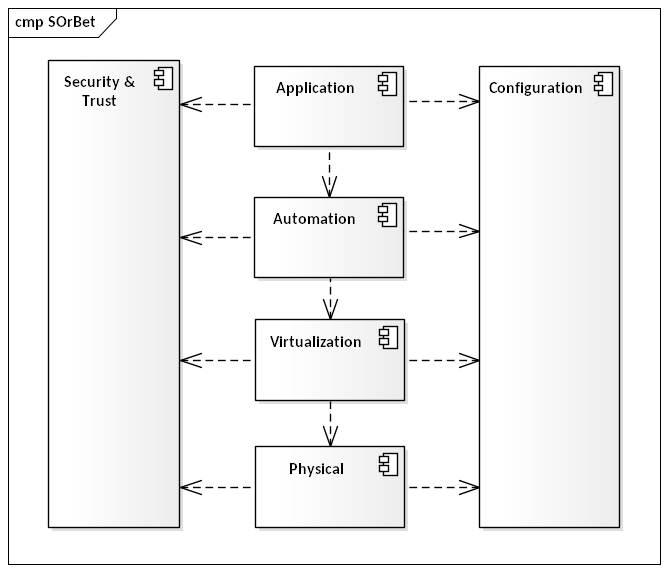
\includegraphics[width=0.8\textwidth]{SorBet.png}
	\caption{SorBet architectural layers}
	\label{fig:sorbet}
\end{figure}

In comparison, the added benefit of SorBet architecture is in concepts of quality of service (QoS) and security. The distinct is also the ability to integrate other applications to use SorBet services, as BMS tend to be practically enclosed. In tailoring for particular inhabitants' rudimentary needs, personal data might be collected that have to be stored confidentially. The other difference to classical BMS is possibly increased dependence of people's lives on minimal downtime and user inability to deal with inexplicable behavior. QoS manager as a part of the virtualization layer provides enough resources and concerns itself with their availability to withstand disruptions.

\section{OpenAIS reference architecture} \label{openais}
Detailed examination of current practices in IoT smart building architectures demands that we consider only one subsystem in isolation, in particular, we deal with lighting control. The methods of its integration with other building systems were already discussed. Open Architectures for Intelligent Solid State Lighting Systems (OpenAIS) set out its primary goal \emph{`to enable a wider community to deliver the smartness of light'} \cite{openais}. This research effort to standardize the luminaries industry segment was funded within Horizon 2020 European Union program \cite{horizon2020}.

OpenAIS serves as a template to develop concrete architectures with multi-vendor and legacy technologies' compatibility in mind. The specification sets out reasonable future-proof guidelines, mainly the use of prospective protocols in intelligent low-powered applications regardless of medium access: IPv6 multicast, 6LoWPAN, LWM2M, DTS. Further, it should enable the transition from the closed and command-oriented lighting control systems towards the Internet of Lighting (IoL). Light as a service being the major driving factor in value chain transformation to bring stakeholders together to benefit from mutual cooperation \cite{iol}. 

The key objectives in coming up with a unified standard for smart lights are several. Firstly it is to define an open architecture with standardized APIs that must be interoperable with building automation systems, cloud services, and other relevant systems. It increases building value by combining IoT, LED technology, and smart grids. Design has to be straightforward to specify, buy, install, maintain and use for stakeholders in the value chain.

Diverse groups operate within the lighing value chain. OpenAIS standard provides relevant viewpoints for the stakeholders (OpenAIS 3.1.3 \cite{openais}):
\begin{itemize}
	\itemsep0em
	\item  \textbf{Logical view}: describes logical functions and their relations, dynamic behavior using message flows and extension mechanisms
	\item \textbf{Physical view}: describes mapping of logical functions to real software and hardware components with categories by resources in execution environments. 
	\item \textbf{Networking view}: conserns itself with communication stack, network protocols and group communication using IPv6 and CoAP multicast.
	\item \textbf{Security view}: lays out requirements based on LWM2M by organizing them according to CIA triad - confidentiality, integrity and availability. Different access rights are assigned based on six-levels of privilege.
\end{itemize}

The logical view decomposes OpenAIS distributed system into components and interfaces in between, separated into two clusters or functional layers. This notion is represented with \textbf{Object Data model} (ODM) as is shown in fig.\ref{fig:openais-odm}. 

\begin{figure}
	\centering
	\begin{subfigure}[b]{0.55\textwidth}
		\centering
		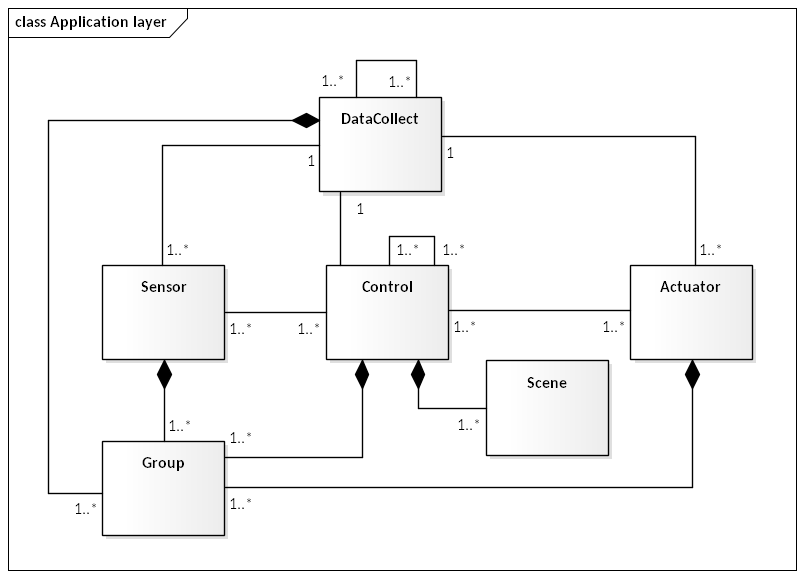
\includegraphics[width=\textwidth]{OpenAIS-Application-layer.png}
		\caption{Application layer}
		\label{fig:OpenAIS-Application-layer}
	\end{subfigure}
    \hfill
    \begin{subfigure}[b]{0.40\textwidth}
		\centering
		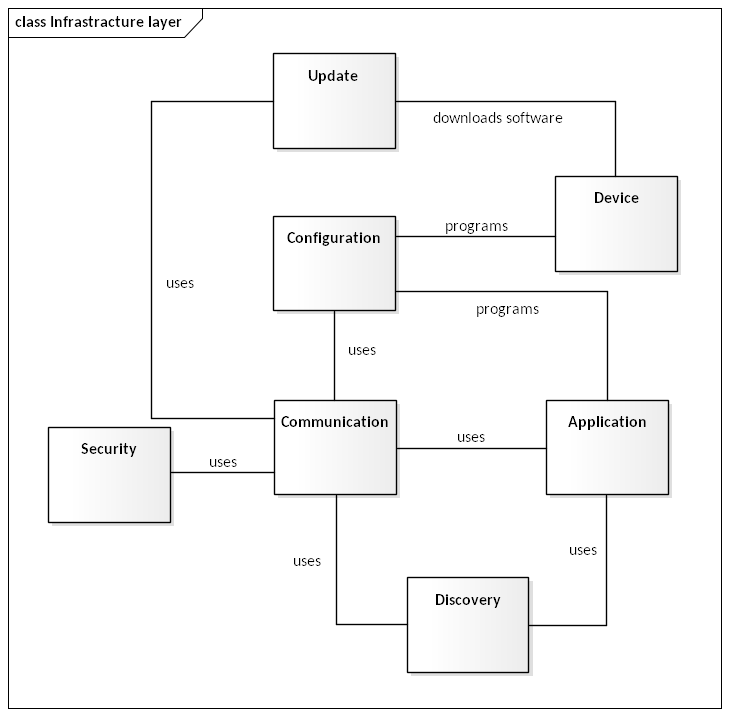
\includegraphics[width=\textwidth]{OpenAIS-Infrastracture-layer.png}
		\caption{Infrastructure layer}
		\label{fig:OpenAIS-Infrastracture-layer}
	\end{subfigure}
	\caption{Object Data model (ODM)}
	\label{fig:openais-odm}
\end{figure}

\textbf{The application layer} (fig.\ref{fig:OpenAIS-Application-layer}) (OpenAIS 3.3.2 \cite{openais}) is made up of a familiar trinity of objects: Sensor, Control, Actuator. In addition, DataCollect supports the collection and storage of occurred events, and the Group object enables multiple of these components to be perceived as an indivisible unit. The scene object coordinates predefined elements in the room to achieve the selected ambiance. 

\textbf{The infrastructure layer} (fig.\ref{fig:OpenAIS-Infrastracture-layer}) (OpenAIS 3.3.3 \cite{openais}) provides for resources and safeguard mechanisms required by the application to properly execute. Each of these objects has to expose the interface as intended by the standard \cite{openais}. There are several types of interfaces: IData produces and sends measurements, IControl executes functions based on caller parameters, IDiscover advertises the presence of component onto the network, and IConfig is responsible for the commissioning and redefinition of algorithmic strategies.

The beneficial idea in ODM is the concept of stacked control to cover up immediate failure, upgrade seamlessly where two versions of the controller can coexist simultaneously, or override lower priority settings. The accessibility of the Device object solely through the Configuration and Update object is similar in some sense to the Virtualization layer in SorBet and abstracts hardware-specific details. This overlay suggests that OpenAIS could be used in IoT distributed control systems unrelated to lighting, e.g. factory assembly line or railway junction switching.

\textbf{The networking view} (fig.\ref{fig:network-stack}) (OpenAIS 3.5 \cite{openais}) is another important architectural piece to compliance with the standard because ODM interfaces are manifested with RESTful API services accessible to the nodes, according to the OMA LWM2M framework. The foundational layer is an IPv6 communication stack with support either wired or wireless. The preferred MAC technology is wired Ethernet and wireless Thread protocol.

\begin{figure}
	\centering
	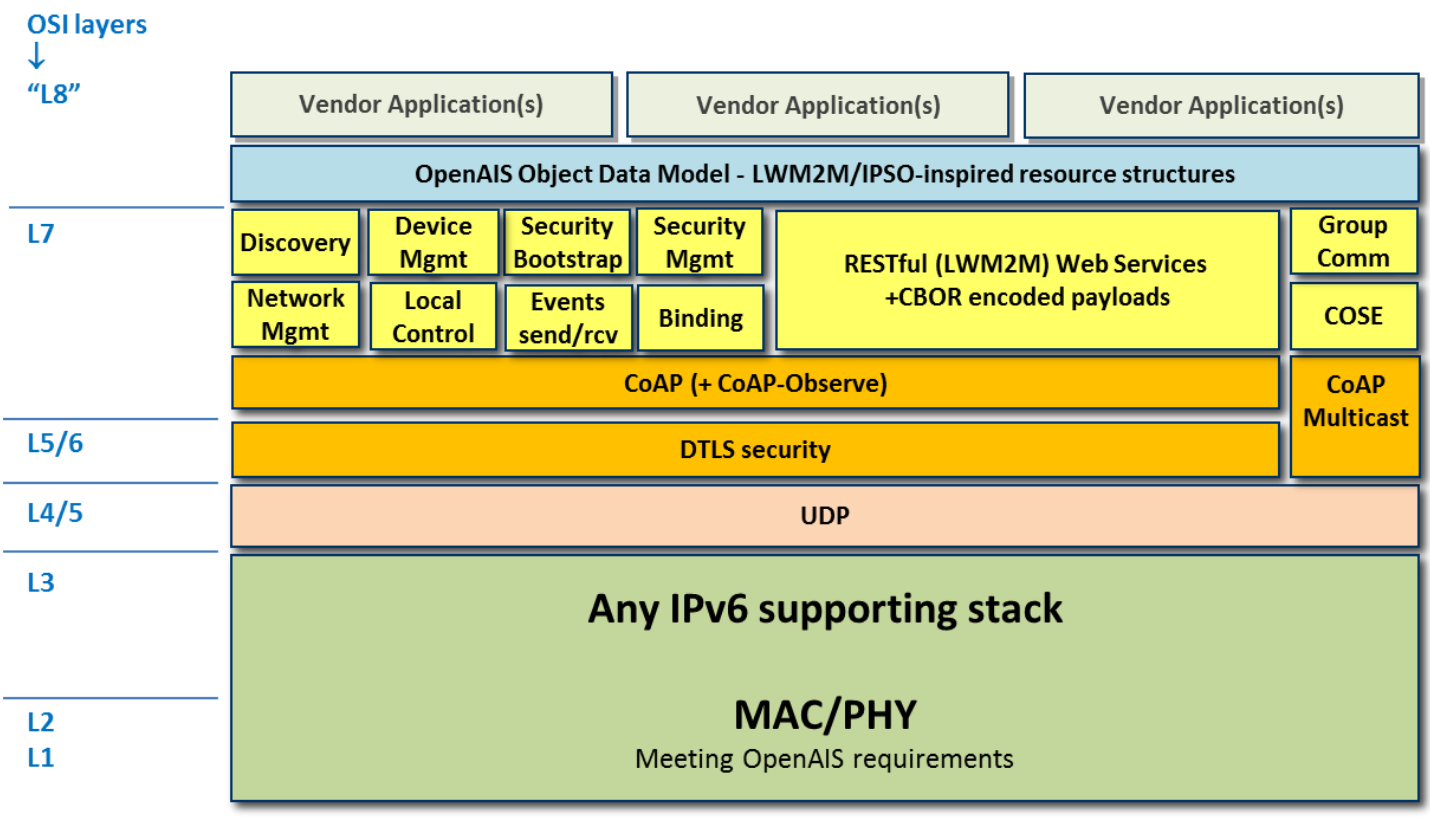
\includegraphics[width=\textwidth]{Network-stack-s-81.png}
	\caption{Network protocol stack}
	\label{fig:network-stack}
\end{figure}

Transport protocol choice with UDP stems from its use in conjunction with CoAP protocol in the target-constrained domain. CoAP optionally supports multicast and observe features to propagate sensor events proactively optimally to larger groups of actuators known jointly as \textbf{Object Group communication} (OGC) (OpenAIS 3.5.6).  Security of unicast datagrams is managed with DTLS. The recommended compact data format is CBOR (RFC7049), instead of JSON.

\begin{figure}[h]
	\centering
	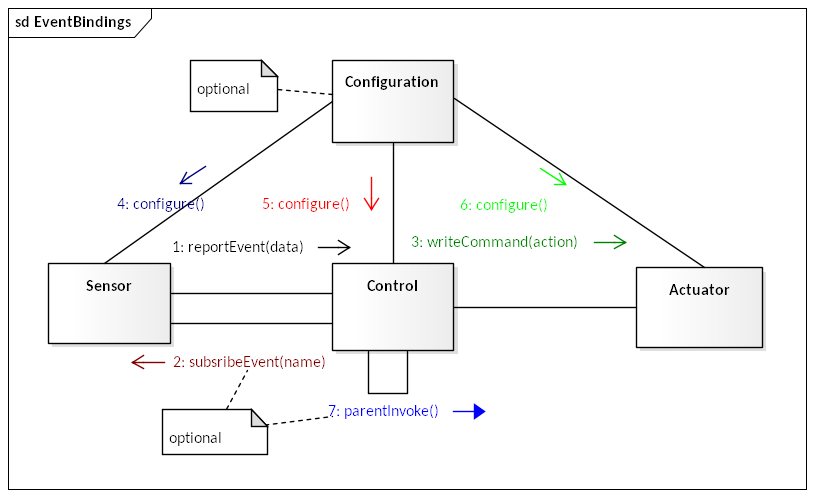
\includegraphics[width=0.8\textwidth]{EventBindings.png}
	\caption{Object Group communication (OGC)}
	\label{fig:ogc}
\end{figure}

The main message flow among the sensor, control, and the actuator is downstream (fig.\ref{fig:ogc}). The controller reacts to sensor events coming in the form of a simple status update with time and sequence number. Sensor event is dependent on originator type but can contain press or no press, presence or no presence, and illuminance brightness. The command generated in the control unit based on the situation aggregated from messages can be either absolute (go to level x), relative (step up x), or relative (scene recall x). Care must be taken to ensure the deduplication of relative commands. Optionally reporting in regular intervals to the controller can be configured.

\section{Illumination scenario simulation} \label{demoapp}
The reference architectures outlined here set out the general structure and boundaries of any real application to be implemented. Therefore our objective is to show how objects' definition from OpenAIS ODM coincides with practical limitations given in the programming language \textbf{Rust}. According to a recent survey and blogs, Rust is becoming more and more popular among IoT enthusiasts because of memory safety and compile-time abstraction \cite{rust-iot} \cite{rust-adoption}. Although wider industry adoption is still a long way away we thought it may be valuable to outline where OpenAIS specification and programming language constructs fell short.

We demonstrate a distributed application simulating the interaction between three key components found in commonplace lighting infrastructures. The focus is to map abstract concepts to the implementation classes. The \textbf{Logical Push-Button} capable of sending \emph{,click'} and \emph{,hold'} events poses as a sensor. It has LWM2M object id of 4002. Emitted messages are directed to a controller which inturn activates each known \textbf{Logical Light-Point Actuators} with an id of 4001. The physical devices are represented by \textbf{FLTK GUI} widgets (fig.\ref{fig:app-rust-gui}). Networking is limited to localhost via selected UDP ports. 

\begin{figure}[ht]
	\centering
	\begin{subfigure}[b]{0.45\textwidth}
		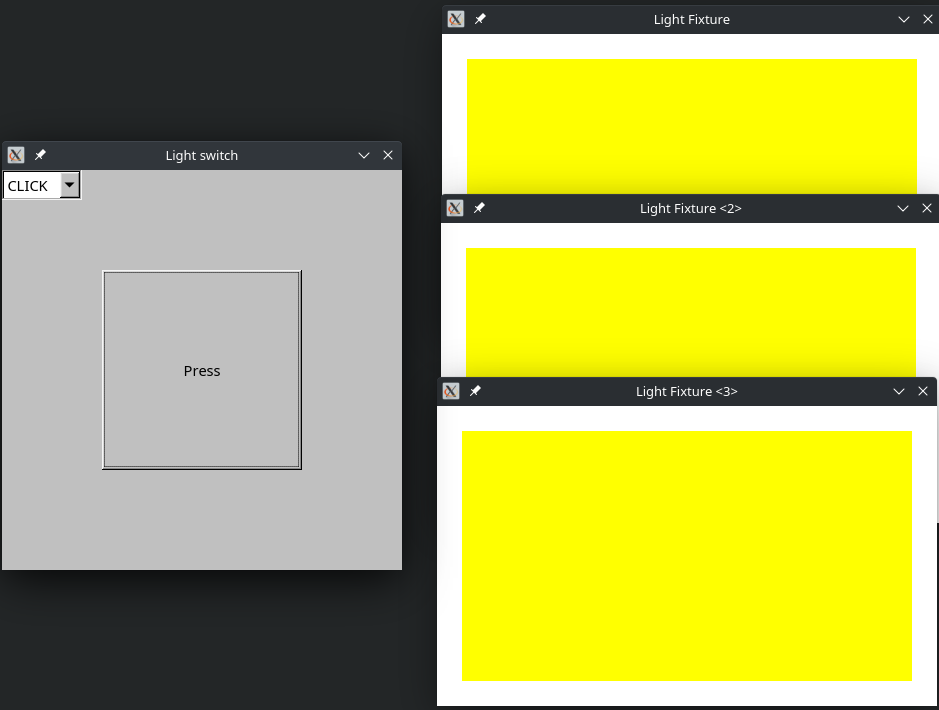
\includegraphics[width=\textwidth]{LightsOn.png}
		\caption{Click event turns light on/off}
	\end{subfigure}
    \hfill
    \begin{subfigure}[b]{0.45\textwidth}
		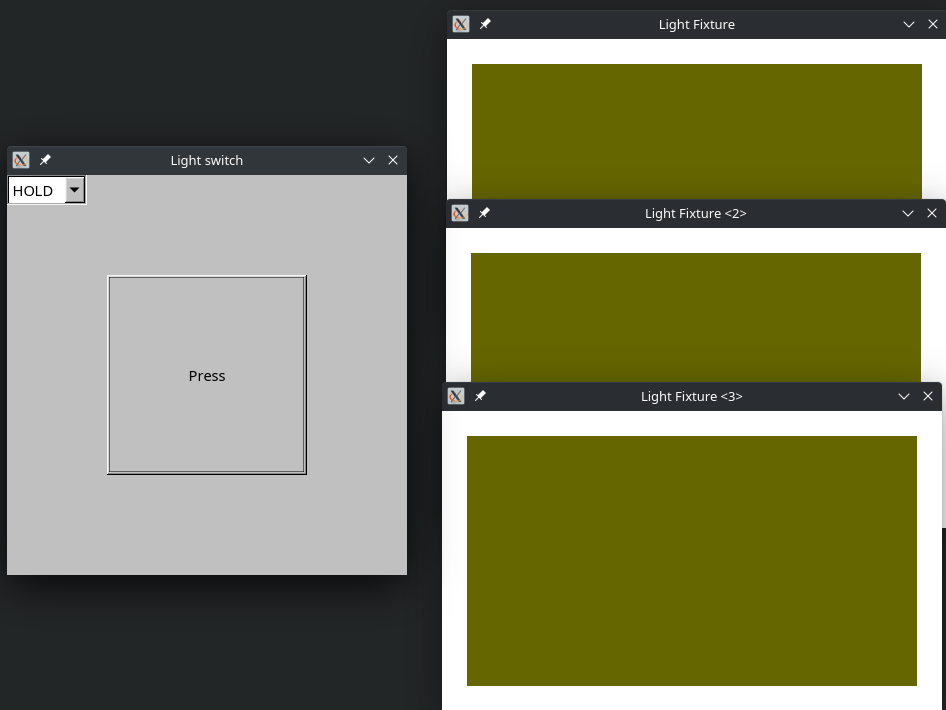
\includegraphics[width=\textwidth]{LightsDim.png}
		\caption{Hold event dims the light ±20\%}
	\end{subfigure}
	\caption{Graphical user interface simulating hardware devices}
	\label{fig:app-rust-gui}
\end{figure}

\subsection{Application composition}
The whole system is partitioned into packages in the way that each component is in a separate package or in Rust's terms it is its own \emph{binary crate} deployable independently (fig.\ref{fig:demoapp-structure}). The Network service is dispatched on incoming request from CoAP server and also encapsulates CoAP client message sending. Besides that it serializes the current state of sensor or actuator to CBOR format. On the other the network service deserializes events and then inkoves correct procedures. 

\begin{figure}
	\centering
	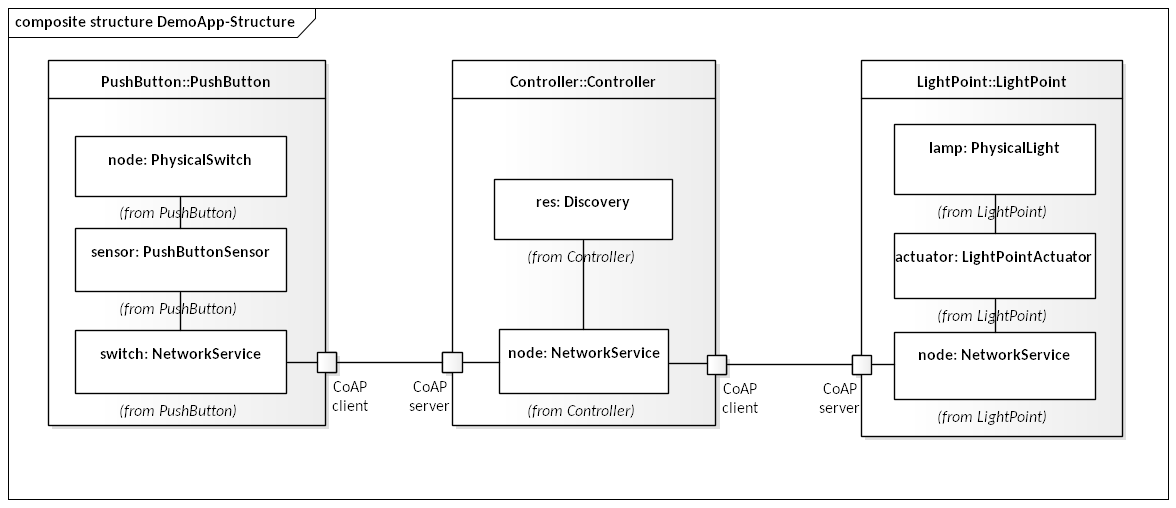
\includegraphics[width=\textwidth]{DemoApp-Structure.png}
	\caption{Simple distributed lighting system overview}
	\label{fig:demoapp-structure}
\end{figure}

The Push button sensor and Light point actuator represents abstraction layer above Physical switch and Physical light. Where as physical devices understands and produces only simple atomic commands which can be binary level alteration after press of the button or output brigthness of a lamp, logical superstructure performs composite effects. 

To illustrate the division of responsibilities we propose an example. Timed dimming in relative steps of 10 \% lasting 2 seconds is activity directed by the Light point actuator, but setting the voltage cap is the job of the Physical light class. Parameters of this action are received and parsed by the Network service. Note that the object of the physical device is a singleton and must be protected by a mutex to avoid light flickering at best and electrical overload damage at worst.

\begin{figure}[ht]
	\centering
	\begin{subfigure}[b]{0.8\textwidth}
		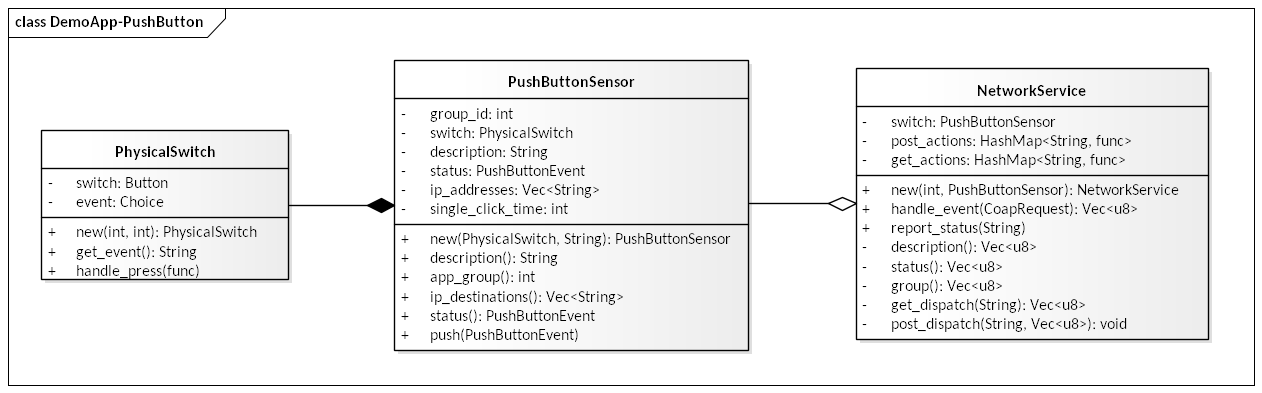
\includegraphics[width=\textwidth]{DemoApp-PushButton.png}
		\caption{Push Button Sensor}
		\label{fig:demo-switch}
	\end{subfigure}
    \hfill
    \begin{subfigure}[b]{0.8\textwidth}
		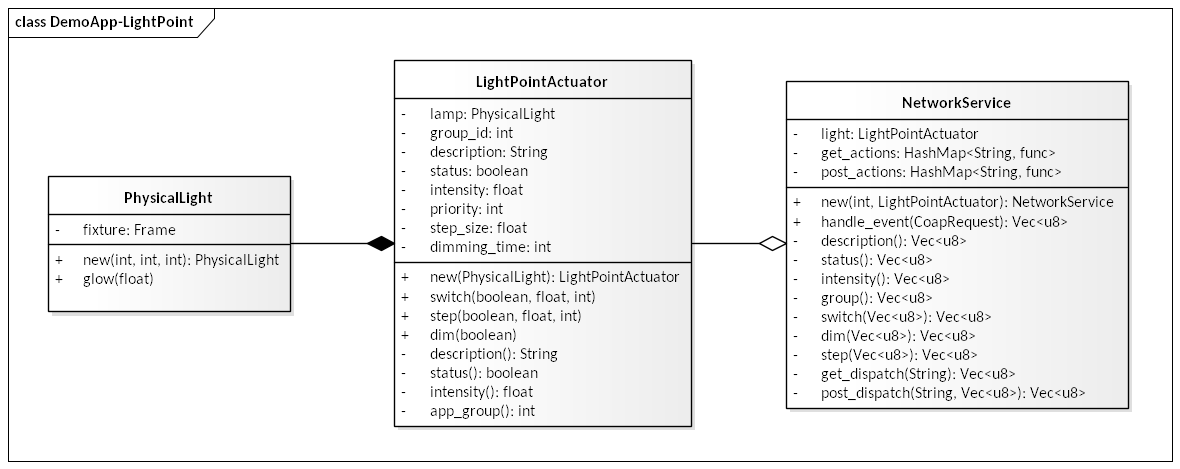
\includegraphics[width=\textwidth]{DemoApp-LightPoint.png}
		\caption{Light Point Actuator}
		\label{fig:demo-light}
	\end{subfigure}
	\hfill
    \begin{subfigure}[b]{0.8\textwidth}
		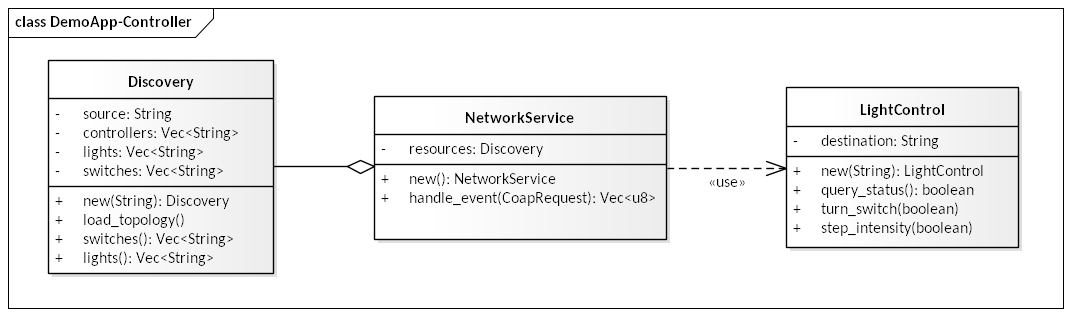
\includegraphics[width=\textwidth]{DemoApp-Controller.png}
		\caption{Controller}
		\label{fig:demo-control}
	\end{subfigure}
	\caption{Class diagrams of the lighting application}
\end{figure}


Validation of this class structure against OpenAIS ODM involves comparing models and finding mutual conformities. Light switch (fig.\ref{fig:demo-switch}) is a Sensor supplemented with included Group from the application layer represented with PushButtonSensor class. In the infrastructure layer, the Communication object matches with the purpose of NetworkSevice, Configuration is realized by PhysicalSwitch, and finally, the Device itself is embodied by GUI widgets. Light fixture (fig.\ref{fig:demo-light}) has the same composition, but instead of Sensor, it utilizes Actuator in LightPointActuator class. 

The controller (fig.\ref{fig:demo-light}) is organized slightly differently because it does not directly interact with any hardware parts. The LightControl class is an implementation of Control with Group object from the model. NetworkService as a Communication object uses Control to send correctly formed messages to actuators listed by the Discovery class with the identical name in ODM. In proper setup, Discovery object would listen to report statuses or heartbeat datagrams in the multicast group. The demo app bypasses this complex error-prone coordination by reading the Yaml file with a static topology list. 

\subsection{Event messaging among components}
CoAP API endpoints that each object must and should implement are defined in the document OpenAIS Appendix A. We do not reach complete conformity with the standard, but the focus remained to provide a minimum viable example and the notable rest is indicated by method prototypes. URL path format to access a single object instance (chosen to be value 1) is as follows: \verb|/s/[object-ID]/[object-instance-ID]/[resource-ID]|. Object ID is a specific type of targeted device, in our case 4001 and 4002, and Resource ID is the function to execute on the service, e.g. 117 is the number to use for switching the light with the POST method.

Because the support of multicast on localhost is nonsensical, CoAP multicast is emulated with the controller sending unicast messages in the loop. Another unfortunate circumstance is the support of clients in blocking mode exclusively. The timeout intervals have to be assigned such that the sensor will wait the whole time until the controller iterates over all registered actuator instances even if none of them respond. 

\begin{figure}
	\centering
	\begin{subfigure}[b]{0.9\textwidth}
		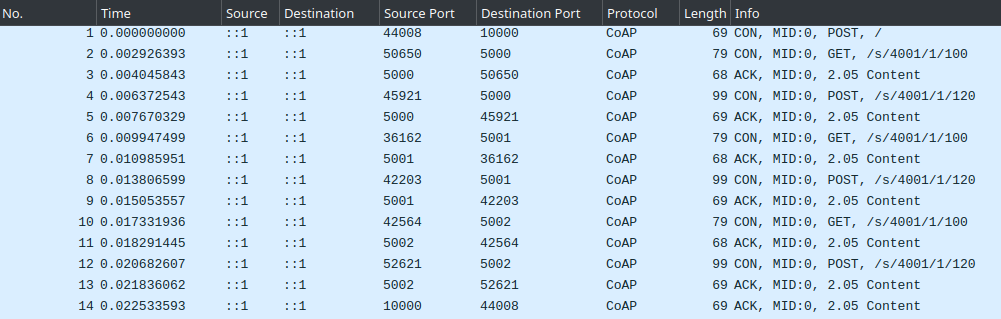
\includegraphics[width=\textwidth]{Dim-light.png}
	\end{subfigure}
    \hfill
    \begin{subfigure}[b]{0.9\textwidth}
		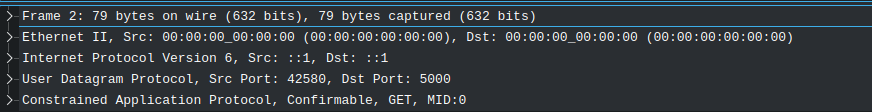
\includegraphics[width=\textwidth]{network-stack-wireshark.png}
	\end{subfigure}
	\caption{Wireshark traces from event messaging among the nodes}
	\label{fig:wireshark}
\end{figure}

The captured packet traces (fig.\ref{fig:wireshark}) show the process of dimming three lights triggered by a button press. The controller on the destination port 10000 is addressed by the first packet. Then for each light point on consecutive ports starting from 5000, the controller requests its current status (with resource id 100) and then dims in the reverse step to switched state (resource 120). When the light is off, it is then brightened by the constant percentage of power. The message flow is dissected by sequence diagrams below (fig.\ref{fig:sequence-button}, \ref{fig:sequence-controller}, \ref{fig:sequence-light}).

\begin{figure}[h!]
	\centering
	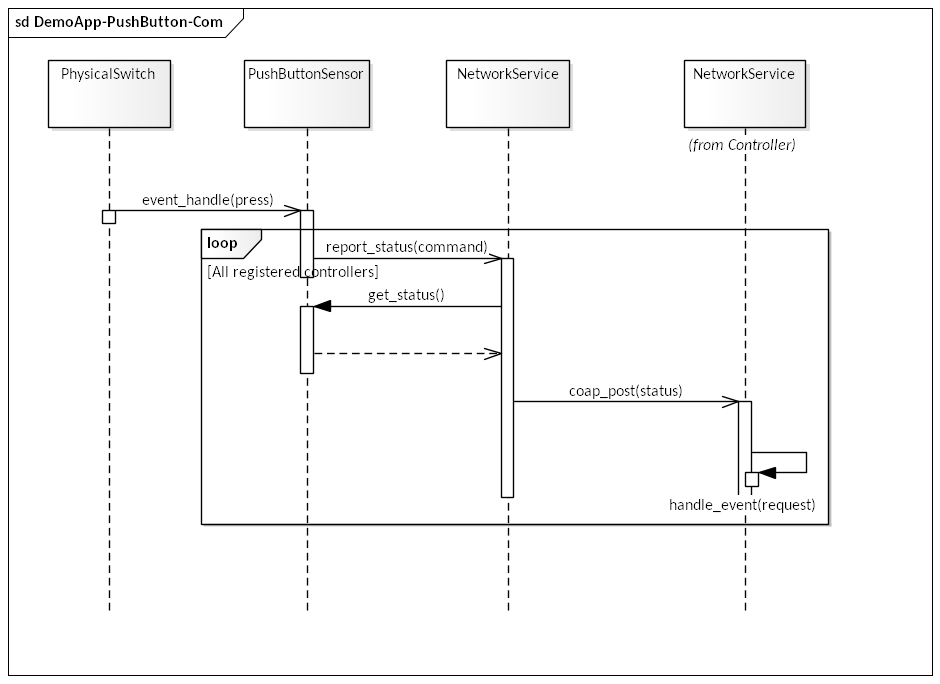
\includegraphics[width=0.8\textwidth]{DemoApp-PushButton-Com.png}
	\caption{Sequence diagram after pressing push button}
	\label{fig:sequence-button}
\end{figure}
\begin{figure}[h!]
	\centering
	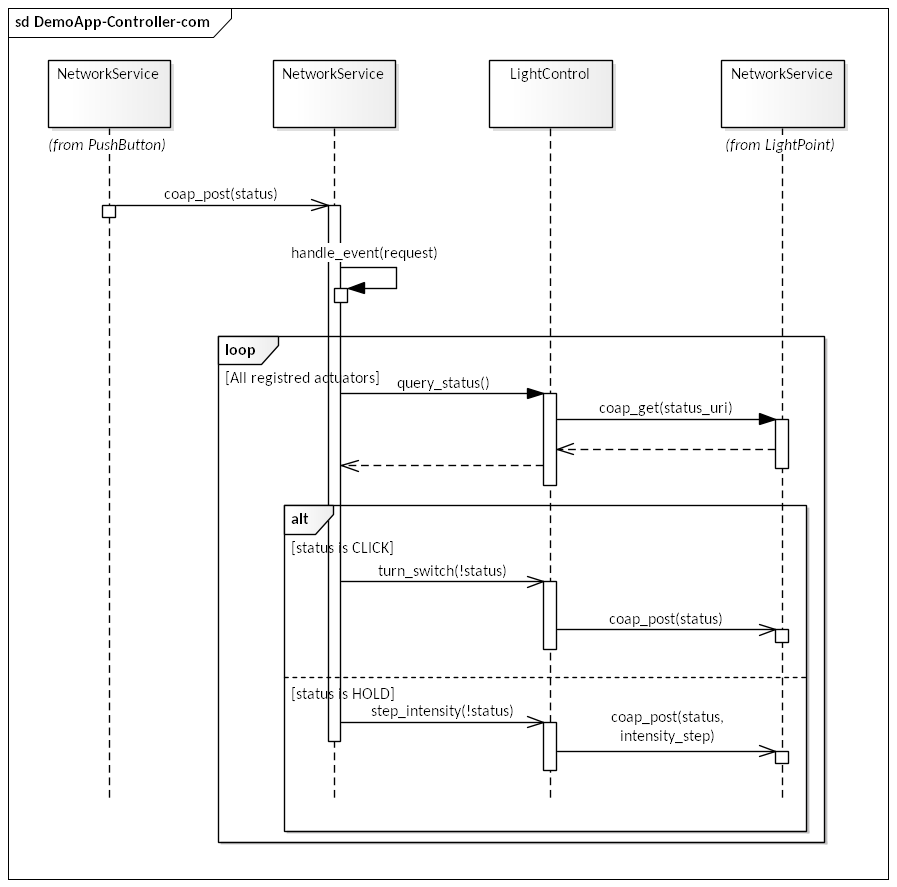
\includegraphics[width=0.8\textwidth]{DemoApp-Controller-Com.png}
	\caption{Sequence diagram of  mediation on the controller}
	\label{fig:sequence-controller}
\end{figure}
\begin{figure}[h!]
	\centering
	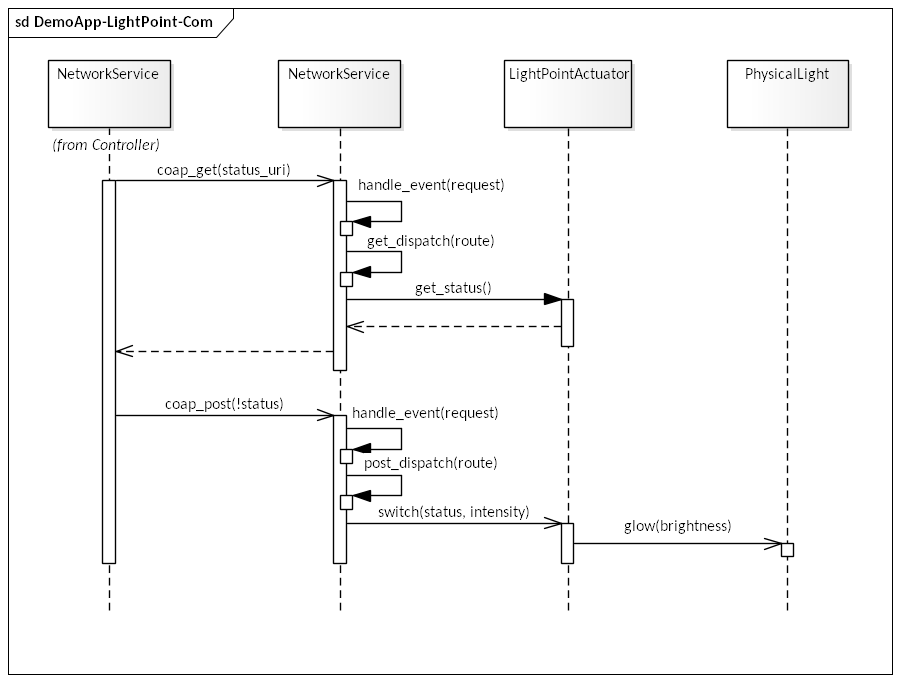
\includegraphics[width=0.8\textwidth]{DemoApp-LightPoint-Com.png}
	\caption{Sequence diagram of turning on illumination}
	\label{fig:sequence-light}
\end{figure}

\subsection{Deployment strategies}
We have to self-critically note that demonstrated sensor network incorporates at the first glance architectural pattern we strive to avoid. Even though implemented sensor-actuator control is centralized it is no coincidence, because it is easiest to develop in this fashion. When there is a need to move components elsewhere it is important to realize that such reorganization can involve only control function, because the sensor and actuator are directly attached to the location of devices.

There are cases when it is better not to further complicate entity organization. Either the controlled regions in question are small enough or split into sufficiently compact blocks. Deployment of this sort when all sensors and actuator messages are routed through the chief unit is labeled area controller (fig.\ref{fig:area-controller}) In corridors lights could be turned on sequentially each section responding to its area controller which means stacked hierarchy is present (fig.\ref{fig:stacked-area-controller}). Nonetheless, in production on the scale, this approach could run into difficulties as a consequence of missing redundancy and significantly increased latency. 

\begin{figure}[h]
	\centering
	\begin{subfigure}[b]{0.45\textwidth}
		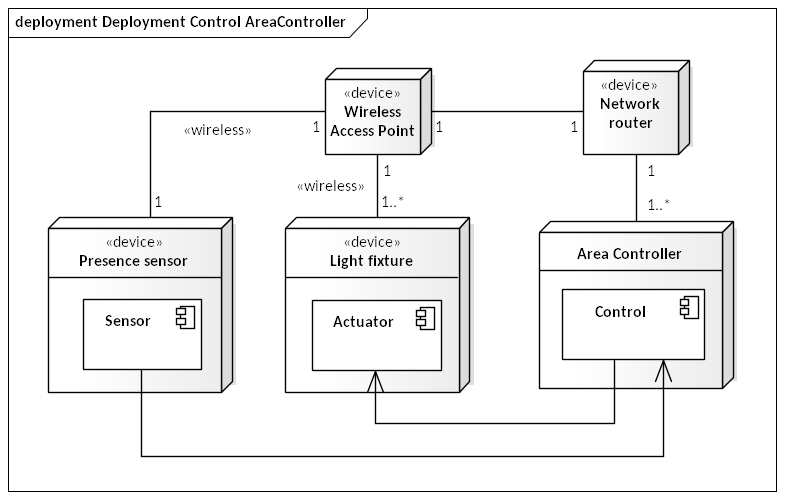
\includegraphics[width=\textwidth]{Deployment Control AreaController.png}
		\caption{Area Controller}
		\label{fig:area-controller}
	\end{subfigure}
    \hfill
    \begin{subfigure}[b]{0.45\textwidth}
		\centering
		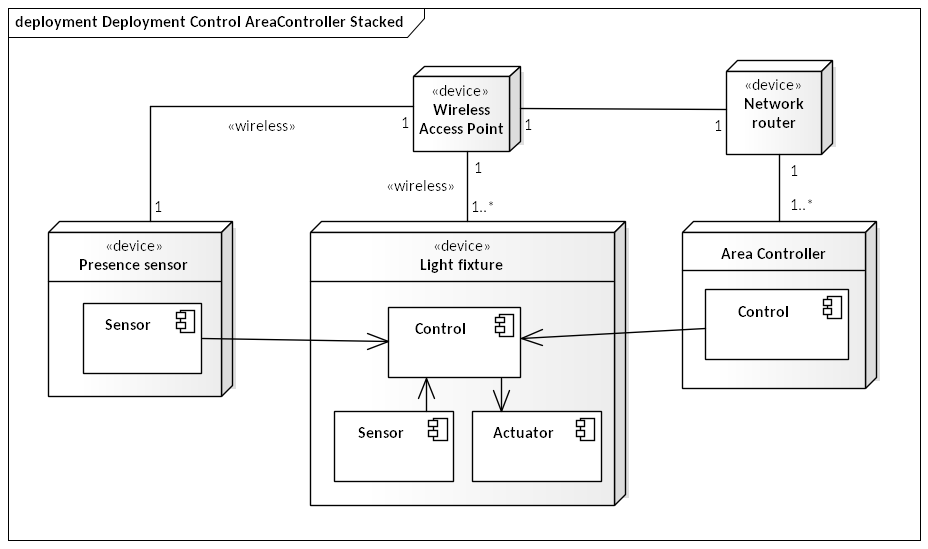
\includegraphics[width=\textwidth]{Deployment Control AreaController Stacked.png}
		\caption{Stacked area controller}
		\label{fig:stacked-area-controller}
	\end{subfigure}
	\hfill
	\centering
	\begin{subfigure}[b]{0.45\textwidth}
		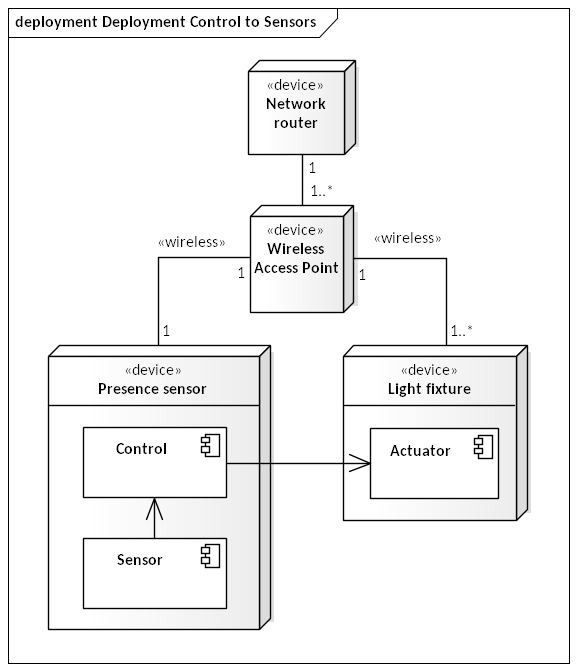
\includegraphics[width=\textwidth]{Deployment Control to Sensors.png}
		\caption{Control to sensors}
		\label{fig:deploy-sensor-controller}
	\end{subfigure}
    \hfill
    \begin{subfigure}[b]{0.45\textwidth}
		\centering
		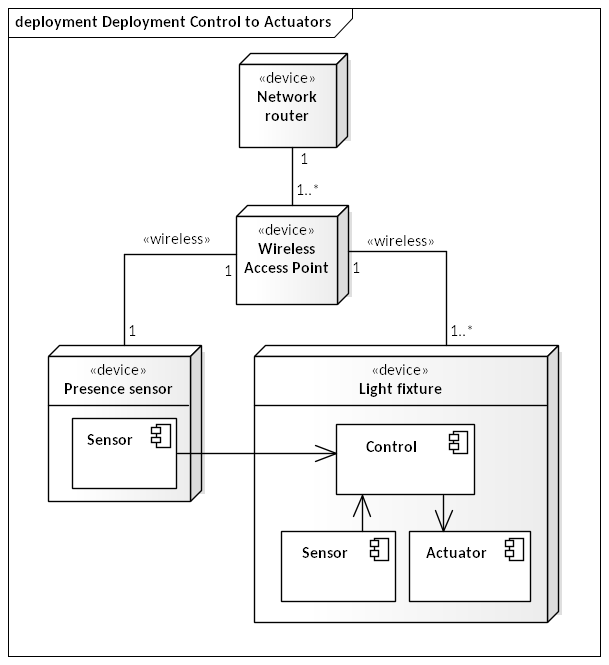
\includegraphics[width=\textwidth]{Deployment Control to Actuators.png}
		\caption{Control to acuators}
		\label{fig:deploy-actuator-controller}
	\end{subfigure}
	\caption{Deployment strategies}
\end{figure}

Among other possibilities is the controllers' distribution to sensor (fig.\ref{fig:deploy-sensor-controller}) or actuator (fig.\ref{fig:deploy-actuator-controller}) nodes. It requires multiplying the control unit which sometimes entails changes in group memberships. In a centralized organization with unicast messaging, as is the case in the proposed illumination scenario simulation, sensor has a record of one outbound IP address for an upstream controller. Whereas controller knows the whole topology. It is practically serving as the message broker. 

Deploying the control unit into sensor devices does not modify groups because it introduces equivalence among sensors. No matter which one is fired action result is lighten up room. In actuator-centered deployment members list exchanges between the sensor and controller. Multicast works analogously just group management is the responsibility of the network router via the MLD (Multicast Listener Discovery) which is IPv6 alternative to IGMP. As for OpenAIS standard it recommends to have small units working independently in case of failure and have fallback to default known state.

\section{Related Work} \label{related-work}
Legacy solutions such as Digital Addressable Lighting Interface (DALI) \cite{sahu_dali_2019} are still operational. New devices should be able to seamlessly incorporate older standards with the use of gateway technology, to allow heterogeneous modularization. DALI is an industrial bi-directional protocol operating on a master-slave two-wire bus. Ballast receives actions to be executed by command words split into frames \cite{dali}.

As a part of the pilot project validation, OpenAIS was deployed in the real office space inside the Witte Dame building in Eindhoven, the Netherlands in 2018. Installation provided for 400 luminaires with embedded sensors across the entire floor. However, source code from their effort is not freely available, but an article on user evaluation was published \cite{openais-pilot}.

\section{Conclusions and Further Work} \label{conclusion}
In this report, we presented two different architectural styles for distributed smart building automation systems: CONDE and SorBet. We evaluated their makeup and event messaging flow patterns as means of integrating control loops to achieve efficient operations and transparent execution of processes. We looked more closely at the lighting in office spaces relatively recently standardized in OpenAIS reference architecture. Based on their design of the Object data model, Object group communication, and recommendations for the networking protocol stack, we implemented a simulation of a communication scenario in Rust programming language. 

The achieved compliance with the standard in the minimal functional example is verified based on finding correspondence between the object model and created classes. We note which components need to be present for each device and the optimal way to achieve separation of concerns on such resource-constrained nodes. The event messaging was analyzed in terms of the efficiency of unicast routing compared to ideal multicast and server limitations in blocking mode. The OpenAIS use for other kinds of IoT solutions is also considered. In the end, the instructions for group membership setup were given based on component placement to physical entities.

The demonstrational app was tested just on one computer. It would be interesting to complete all the mandatory requirements to create a fully-fledged open-source example for OpenAIS which can prove as a useful infrastructure in verifying vendor-developed services. Modularity may be also examined whether it suffices to change the Physical device class to interface with the hardware or other supporting functionality or whether a more substantial modification of the current structure is necessary. 
 
\printbibliography
\end{document}